\begin{figure*}[t]
\centering
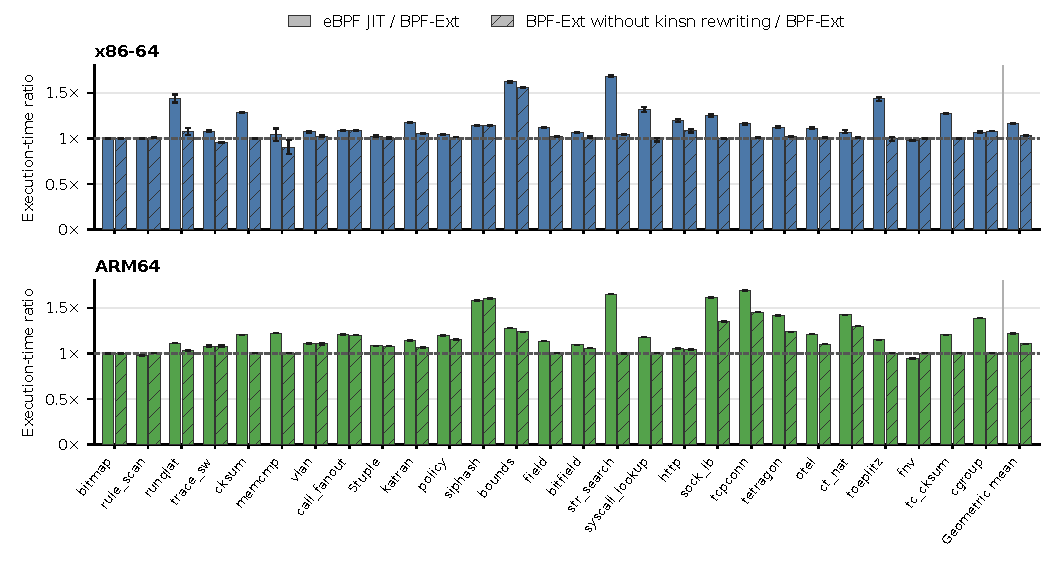
\includegraphics[width=\textwidth]{figures/sec-6-micro-performance.pdf}
\caption{Execution-time ratios for the microbenchmarks in Table~\ref{tab:microbenchmarks}. Ratios are the reference configuration's mean execution time divided by that of \tool{}. Values above 1 indicate faster execution with \tool{}. Disabling \kinsn rewriting preserves the LLVM configuration. Geometric mean summarizes the 27 ratios. Error bars show 95\% confidence intervals from paired resampling of independent instances.}
\Description{Two panels show execution-time ratios for x86-64 and ARM64 across 27 benchmarks and their geometric means. Solid bars compare eBPF JIT with BPF-Ext. Hatched bars compare BPF-Ext without kinsn rewriting with BPF-Ext. The dashed horizontal line marks equal execution time.}
\label{fig:eval-kinsn-micro}
\end{figure*}